\documentclass[conference]{IEEEtran}
\usepackage{algorithm}
\usepackage{algpseudocode}
\usepackage{amsmath}
\usepackage{graphicx}
\usepackage{tikz}
\usepackage{hyperref}
\usepackage{multirow}
\usepackage[center]{caption}
\usetikzlibrary{shapes,arrows,automata,positioning}
\tikzset{>=latex}
\tikzstyle{cloud} = [draw, ellipse, node distance=1.5cm,
    minimum height=2em]

\setlength{\belowcaptionskip}{-10pt}

\title{An Autonomous Meeting Assistant}
\author{951926 \and 1001231 \and 1024072 \and 1028907}
\date{\today}

\begin{document}
\maketitle

\begin{abstract}
In this report, we present a system which performs the 1996 AAAI Mobile Robotics Competition task ``Call a Meeting''\cite{AAAIcomp}. The robot was tasked with finding a meeting room, ensuring it is empty and bringing a certain number of people to the room within a 15-minute time limit. To complete the task, we use probabilistic roadmapping, Monte Carlo localisation and a face detection module using the ROS framework, installed on a laptop, mounted on a Pioneer 3-DX platform modified with a tripod-mounted Kinect.
\end{abstract}
\section{Introduction}
Solutions to complex tasks often require the use of multiple techniques to solve different sub-problems, and this task is no exception. We were required to implement a localisation algorithm to determine the position of the robot, a probabilistic roadmap to allow paths to be planned through the space, a navigation algorithm for path planning, a method of exploring the space, and some way of detecting people. We then had to implement a system which would combine all of these separate modules into a single system that would complete the task. In the next section we present some background information about techniques that are often used to solve these sorts of problems. We then provide a detailed description of our system, before evaluating its performance and discussing experimental results. Finally, we conclude and suggest areas for improvement.

\section{Background}
In this section, we discuss briefly the areas of robotics that are relevant to solving the task that has been set. We mention specific algorithms and techniques that we considered using, as well as describing briefly the benefits and drawbacks of some of the techniques.

\subsection{Localisation}
The aim of localisation is to obtain an estimate of the position of a mobile robot using sensor data \cite{localisation}. While it is possible to use odometry data to do so, this data is inherently noisy and prone to error. In particular, odometry errors can arise from changes in the surface the robot is travelling across and the robot's weight. An important point to note is that localisation can be performed with a pre-defined map, as well as by generating a map in real-time. The much more complex latter problem is called simultaneous localisation and mapping (SLAM), which we will not discuss here. See \cite{slam} for an introduction to the SLAM problem.

\subsubsection{Bayes Filter}
Many advanced localisation techniques are based on the Bayes filter, shown in Algorithm \ref{alg:bayesfilter}, which uses a belief distribution $bel(x_t)$ to represent the state $x_t$. The calculation of $bel(x_t)$ at time $t$ is dependent on $bel(x_{t-1})$ at time $t-1$, the last action $u_t$, and the last measurement $z_t$. In the first step, called the prediction step, the prior belief $\overline{bel}(x_t)$ is calculated. This step merges two probability distributions; the prior belief over the previous state $x_{t-1}$, and the probability of transitioning from that state to the posterior state $x_t$ given that the action $u_t$ was taken. This step does not take into account any measurement taken in the posterior state, predicting using only
the knowledge of the action taken. In the second step, the measurement update, the posterior belief is calculated by multiplying the prior belief with the probability of being in the posterior state given that the measurement $z_t$ was observed. The result of this multiplication is generally not a probability, and therefore requires normalisation using some constant $\alpha$. As there are usually multiple posterior states, $x_t$ is usually a state vector rather than a single state, and so the two steps will be applied multiple times in order to update the belief for each state being considered. The filter is recursive, requiring some idea of the initial belief $bel(x_0)$ at time $t=0$. The initial belief is either a distribution centred on $x_0$, in the case where the initial position is known, or a uniform distribution over the space otherwise.
\begin{algorithm}
  \caption{Bayes filter \cite{thrun}}
  \label{alg:bayesfilter}
  \begin{algorithmic}[1]
        \State \textbf{Algorithm Bayes\_filter}\textnormal{($bel(x_{t-1}), u_t, z_t$)}
        \For{\textnormal{all} $x_t$}
        \State $\overline{bel}(x_t)=\int P(x_t\mid u_t, x_{t-1})bel(x_{t-1})dx_{t-1}$
        \State $bel(x_t)=\alpha P(x_t \mid z_t)\overline{bel}(x_t)$
        \EndFor
        \State \Return $bel(x_t)$
  \end{algorithmic}
\end{algorithm}
As the Bayes filter is not restricted to finite state spaces, it is not possible to implement it for anything other than very simple problems. There are two families of algorithms for localisation, known as \emph{recursive state estimators}, with various properties that permit the use of the Bayes filter in more complex estimation tasks \cite{thrun}.
\subsubsection{Gaussian Filters}
The basic principle of the family of Gaussian filters is the use of multivariate normal distributions, which can be formulated from a mean $\mu$ and covariance $\Sigma$, to represent belief. As a result, the assumption that the system is a linear Gaussian system is made; the initial belief must be a Gaussian, and both the state transition function and measurement probability must be linear functions. Although Gaussian filters can be extended to non-linear systems, they perform best when the system meets the assumptions made. One of the main advantages of such filters is the computational complexity, which is polynomial with respect to the dimensionality of the state space. The main disadvantage is that Gaussians are unimodal and therefore cannot represent situations in which there are multiple hypotheses; a situation that is often encountered in robotics. Examples include the Kalman filter and the information filter, which are derived from two different ways of representing Gaussians. Both of these filters can be extended to non-linear systems by using a Taylor expansion to produce linear approximations of non-linear functions. Mixtures of Gaussians can also be used to extend the Kalman filter to encompass situations in which multiple hypotheses are required, but each extension increases the complexity of the algorithm. This extensibility is one of the reasons for the popularity of the Kalman filter in state estimation problems. With some extension, the information filter is particularly suited to multi-robot systems where information from multiple sources must be integrated, but issues with complexity have resulted in the Kalman filter becoming the more popular of the two for the majority of problems \cite{thrun}.

\subsubsection{Nonparametric Filters}
In contrast to Gaussian filters, nonparametric filters discretise the probability distribution and do not require assumptions of linearity and Gaussian belief distributions. Instead, the state is approximated by a finite number of values which are taken from the belief state at any given time. The number of these values can be varied, and nonparametric filters converge to the correct state as the number tends towards infinity. Because this family of filters does not impose restrictions on the posterior density, they are useful for problems such as global localisation, which require the state to be represented in a complex form. Global localisation is the problem of determining the position of the robot without knowing its initial position, resulting in global uncertainty and the need for a multimodal belief distribution. Although as a result nonparametric filters are more computationally expensive than Gaussian filters, it is possible to vary the number of values used to represent the belief to suit the problem using \emph{adaptive} techniques. Examples of these types of filters are the histogram and particle filters. The histogram filter decomposes a continuous space into some finite number of regions, each of which is assigned a probability based on the belief. Extensions include using dynamic decomposition techniques to use more coarse representations in regions with lower probability, and the use of \emph{selective updating}, which updates only the parts of the space which are deemed important. Particle filters approximate the belief by drawing a number of hypotheses called \emph{particles} randomly from the belief distribution. The most important part of the particle filter is the resampling step, which selects particles from the initial set proportional to an importance factor. This has the effect of concentrating particles in areas of high likelihood, reducing computational power spent in areas which are not relevant. Improving the sampling method and adapting the number of particles based on time and uncertainty lead to more effective and error-resistant particle filters. A property which is particularly useful to us is that particle filters are very easy to implement \cite{thrun}.

\begin{algorithm}
  \caption{Basic Monte Carlo Localisation \cite{thrun}}
  \label{alg:basicMCL}
  \begin{algorithmic}[1]
    \State \textbf{Algorithm MCL}\textnormal{($\mathcal{X}_{t-1}, u_t, z_t, map$)}
    \State $\bar{\mathcal{X}}_t=\mathcal{X}_t=\emptyset$
    \For{$m=1$ to $M$}
    \State $x_t^{[m]}=\textbf{sample\_motion\_model}(u_t,x_{t-1}^{[m]})$
    \State $w_t^{[m]}=\textbf{sensor\_model}(z_t,x_t^{[m]},map)$
    \State $\bar{\mathcal{X}}_t=\bar{\mathcal{X}}_t+\langle x_t^{[m]},w_t^{[m]}\rangle$
    \EndFor
    \For{$m=1$ to $M$}
    \State \textnormal{draw $i$ with probability $\propto w_t^{[m]}$}
    \State \textnormal{add $x_t^{[i]}$ to $\mathcal{X}_t$}
    \EndFor
    \State \textbf{return} $\mathcal{X}_t$
  \end{algorithmic}
\end{algorithm}

\subsubsection{The Markov Assumption}
One of the reasons that these filters are so efficient stems from the assumption that the Markov property holds. While this may not actually be the case, the Bayes filter that forms the base of these filters is robust to the violation of some of the requirements of the property. The Markov property states that the future states of the system do not depend on past states. In other words, considering all previous states of the system provides no additional information for predicting future states; all prediction can be done using only the current state. Previous states do not have to be included in calculations, and as a result do not need to be stored, which leads to faster computation and lower memory usage.

\subsubsection{Sensor \& Motion Models}
To use any of these filters to solve a localisation problem, it is necessary to model the sensors and motion of the robot. These models include some parameters representing the uncertainty attached to performing a specific action or receiving a certain measurement from a sensor. The motion model is used in the prediction step to determine the state transition probability $P(x_t\mid x_{t-1}, u_t)$; the probability of going from state $x_{t-1}$ to $x_t$ given that the action $u_t$ was performed. The sensor model is used to calculate $P(z_t\mid x_t,map)$, which represents the likelihood of the measurement $z_t$ being received in the state $x_t$ on a given map. The model incorporates knowledge about the noise parameters of the operating environment and the sensor being used in the form of probability densities. For example, a range sensor could include densities for correct measurements, measurements of unexpected obstacles, sensor failures and random measurements \cite{thrun}. 

Integrating the sensor and motion models into the particle filter results in an algorithm known as Monte Carlo localisation (MCL). The most basic version of MCL is shown in Algorithm \ref{alg:basicMCL}, in which $\mathcal{X}_{t-1}$ represents the particles from the previous time step, $M$ the total number of particles, $x_t^{[m]}$ the state of the $m$th particle with the action $u_t$ applied to it via the motion model, $w_t^{[m]}$ the importance weight of the $m$th particle, and $\bar{\mathcal{X}}_t$ the resampled set of particles. We use an adaptive implementation of MCL provided by the ROS system.
\begin{figure}
  \centering
  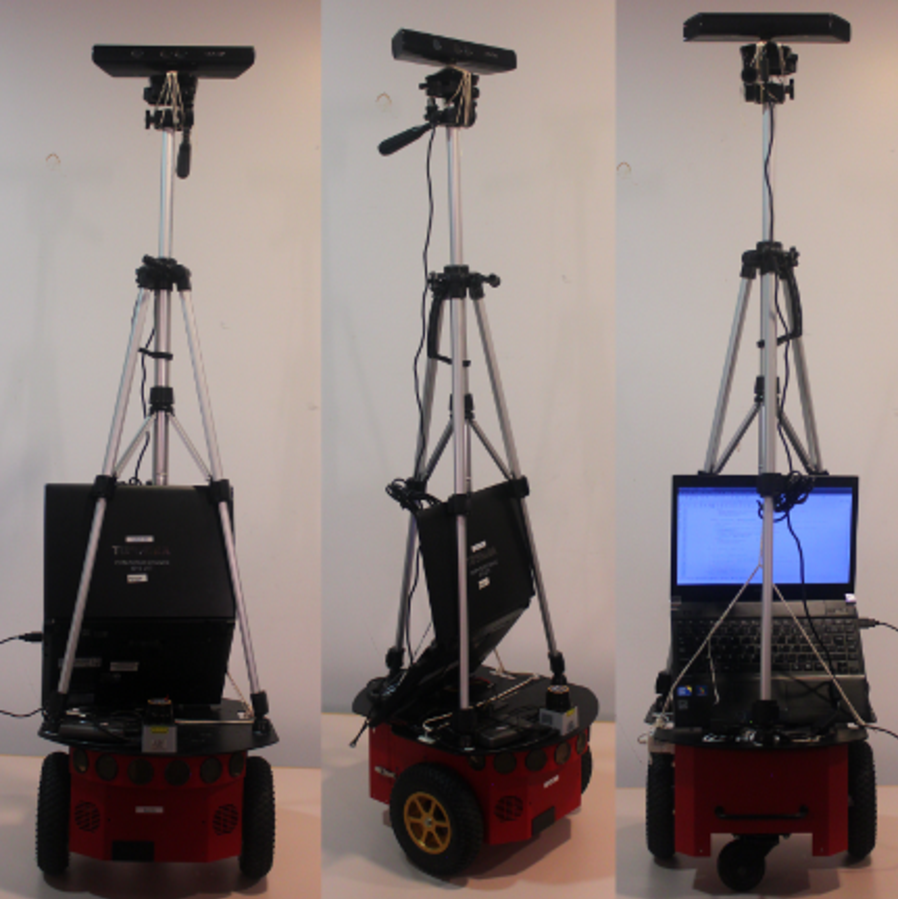
\includegraphics[width=\columnwidth]{robotmulti}
  \caption{The Pioneer 3-DX fitted with tripod mounted Kinect and Hokuyo laser rangefinder.}
  \label{fig:robotpic}
\end{figure}
\subsection{Route Planning}
\subsubsection{Probabilistic Roadmaps}
A probabilistic roadmap (PRM) is a  multi-query motion planning algorithm for robots in static workspaces \cite{prm} which solves the problem of determining a path between start and goal configurations while avoiding collisions with obstacles in the workspace. The roadmap algorithm consists of two phases; the learning phase and the query phase.

In the first step of the learning phase, the construction step, a graph $G$ with vertices $V$ and edges $E$ is constructed. Free configurations are repeatedly sampled from the workspace and added to $V$. A free configuration is one where the robot does not intersect with walls or other obstacles in the workspace. Once a specified number of configurations have been sampled, the vertices in $V$ are connected. Attempts to connect two vertices $v$ and $n$ are only made if they are within a neighbourhood specified by a maximum distance $D$, and a connection is only made if the path between the two vertices is also valid, i.e. there is no configuration on the path where the robot intersects with walls or obstacles. If a connection is made, the edge from $v$ to $n$ is added to $E$. The second step of the learning phase is the expansion step, which is intended to improve the connectivity of the graph. This step can be skipped if a sampling algorithm, which takes into account difficult (narrow) areas of the workspace, is used in the construction step.

Once the graph has been constructed, the query phase is entered. In this phase, the roadmap is used to find paths between the start and goal locations $s$ and $g$. In order to do this, $s$ and $g$ must first be connected to the graph using the same connection strategy used in the construction step. A graph search algorithm, such as A*, can then be used to find the shortest path between the two newly added vertices.

There are a number of ways in which the basic PRM algorithm can be improved. Most of these relate to the construction of the graph, as the graph is the part of the algorithm which most influences subsequent performance---if vertex placement is bad, then even with a good graph search algorithm, it is possible that a path will not be found. The sampling method is particularly important, and many different techniques have been proposed to improve the coverage of the PRM. Roughly speaking, the techniques can be separated into uniform and advanced techniques. Uniform techniques include random sampling, sampling points on the intersection points of a grid, and splitting the workspace into cells and sampling some number of points from each of those subspaces. Uniform methods provide a simple but effective way of sampling, but may experience a drop in performance for more difficult workspaces, for example those with narrow corridors. In these cases, using advanced techniques such as medial axis sampling, which generates points at the midpoints between obstacles, can be effective \cite{sampling}. The strategy used to connect vertices can also affect the structure of the graph, which in turn affects the query phase. Improvements to the query phase can be made by using different graph search algorithms, but unless the graph is extremely dense, the query time is negligible. As an example, our implementation of Dijkstra's algorithm took 964 milliseconds to find a path between two points on opposite sides of the map with a roadmap populated with 5000 vertices. A path smoothing technique (our implementation can be found in Algorithm \ref{alg:pathsmooth}) can also be used on the path found by the graph search algorithm to improve it further. In some cases, a path may not be found with the graph being used, and although expensive, re-generating the graph can sometimes remedy this problem.

\subsubsection{Rapidly Exploring Random Trees}
A Rapidly Exploring Random Tree (RRT) is a randomised data structure and algorithm that is also used to solve path planning problems. RRTs are designed to handle nonholonomic constraints and high degrees of freedom \cite{rrt}. Instead of sampling points and then attempting to connect them as in PRMs, RRTs are biased towards moving into unexplored areas of the state space by sampling points and being ``pulled'' towards them \cite{rrtprog}. There are several planners for RRTs, including a bidirectional planner where the tree grows from the start and goal vertices and uses an aggressive heuristic to connect the trees. In contrast to the multi-query PRM, an RRT is a single query algorithm; it is rerun every time a query is made. The properties of RRTs make them particularly suited to problems involving robot arms and robots with nonholonomic kinematics. As our platform can be considered holonomic, we mention RRTs for completeness.

\subsection{Exploration}
The problem of exploration involves taking action to maximise information gain, given the current knowledge of the world. What is meant by information gain depends on the problem being solved. In many cases this is discovering the locations of walls and obstacles, but can also extend to more complex objectives such as determining the locations of specific objects, rooms and people. The most basic form of exploration is the random walk, which ensures that any finite sequence of actions will be executed eventually \cite{thrunexploration}. However, this is a drawback as it is an exhaustive search, and many other improved exploration techniques have been proposed. Greedy techniques move the robot from its current location to the closest location that has not yet been explored \cite{greedy}. Frontier-based exploration moves to boundaries between open space and uncharted territory in order to maximise its information gain \cite{frontier}. Distributed approaches using coordinated multi-robot systems have become an active area of research, and novel techniques drawing on concepts from economics have been proposed \cite{multiexp, marketexp}. As with many solutions using distributed computing, the use of multiple ``processors'' allows the task to be completed in a shorter time, but requires the implementation of algorithms that can make good use of these increased capabilities.

\subsection{Face Detection}
Face detection is concerned with finding whether or not there are any faces in a given image (usually in gray scale) and, if present, return the image location and content of each face \cite{yang2008face}. Research in this field can be dated back to the early 1970s, when a number of techniques such as simple heuristics and anthropometric techniques were proposed \cite{hjelmaas2001face}. However, these techniques were not very adaptable to changes in the environment, requiring either a lot of tweaking or complete system redesigns. Face detection techniques can be broken down into two separate groups, feature-based and image-based \cite{hjelmaas2001face}. Feature-based approaches tend to make use of facial features such as facial geometry and skin colour to detect faces. An example of a feature-based approach are Haar-like features, which use contrast variances between adjacent rectangular groups of pixels to classify objects and faces by combining them to make features. Image-based face detection does not have knowledge regarding features presented to it, instead using training and mapping techniques to build detection systems. Neural networks, which use training samples to build up a classification system to identify faces, are an example of an image-based approach. For our system, we considered two particular methods of face detection. One of the methods is known as blob detection which uses a method to extract adjacent regions of the same colour to identify as an object. The other method, which we eventually chose to use, was Haar cascades, face detection using Haar-like features. The way in which this classifier works is by using the change in contrast values between adjacent rectangular groups of pixels, as opposed to using intensity values of a pixel \cite{wilson2006facial}. Contrast variances between pixel groups allow relative light and dark areas to be determined, where two or three adjacent groups with a relative contrast variance form a Haar-like feature. Due to the large number of features which can be derived, a system can be trained to find the best set of features which can then be combined in order to produce a classifier cascade \cite{viola2004robust}. In the detection phase for a face, a window of a specific size is moved over the input image. A classifier cascade containing all of the Haar-like features is applied to each region of the image which falls within the window, and successful classifications within this window are used to determine whether a face is present in the region.

\section{Design}
In this section we explain in detail the techniques, algorithms and hardware that we used to solve the task.
\subsection{Hardware \& Software}
\subsubsection{Robotics Platform}

For the task, we used a Pioneer 3-DX fitted with a Hokuyo URG-04LX laser rangefinder. The Pioneer is 455mm long, 381mm wide, 237mm high, and weighs 9kg, making it a relatively compact platform. It is fitted with six front-mounted and two side-mounted sonar sensors. The robot is powered by three batteries which provide a run time of 8-10 hours, assuming no accessories are attached. The robot is equipped with a differential drive system which has a 0cm turn radius, so it can be considered holonomic. The maximum translation and rotation speeds are 1.2m/s and 300$^\circ$/s respectively \cite{pioneer}. 

The Hokuyo laser is mounted on the front of the robot. It has a scan area of $240^\circ$ with a maximum radius of 4m and an angular resolution of $0.351^\circ$. A scan is completed by the laser every 100ms. The laser is accurate to $\pm 20$mm at distances between 20 and 1000mm, and $\pm 1$\% of the measurement distance at 1000-4000mm \cite{hokuyo}.

The Microsoft Kinect is a video device which produces colour images much like a normal camera, but has the additional ability to return a distance (depth) value for each pixel in the image. As such, the device is similar to a 3D camera. The Kinect camera has a $57^\circ$ horizontal and $43^\circ$ vertical field of view with a nominal depth of 3.5m. Images from the camera have a resolution of 640x480 \cite{Kinect}. Interfacing the Kinect with the ROS framework is achieved by using the OpenNI SDK, an open source framework for 3D sensing development.
\subsubsection{Robot Operating System}
The Robot Operating System (ROS) is an open source software framework developed by Willow Garage and the robotics community that provides libraries and tools for use in robot applications. The system comes with a series of \emph{stacks}; user-contributed packages which can be used to perform SLAM, localisation and various other common tasks, which means that development can be focused on solving the problem at hand. ROS development can be done in a variety of programming languages, including C++, Python and Java, and can be run on a large number of platforms, with support for humanoid robots, arms, quadrotors and many mobile robots.

The system has a graph-like structure and makes use of data streams for communication between nodes, and as a result is robust to node failures. The use of data streams for communication allows for a high degree of modularity---a node written for one task can be used in the system for another task with little or no modification. Each node can have an arbitrary number of \emph{publishers} for sending messages to \emph{topics} and \emph{subscribers} for receiving them. One of the major strengths of the system is that when a message is sent, it does not have to be sent to a specific node; once it is published, the message is available to any node which is subscribed to the topic on which it is published. A  master node provides information about the state of the whole system, including node status and the currently active topics.

\subsection{System Structure}
Our implementation attempts to make the most of the ROS system, with separate nodes for each subsystem. The actions of the system are controlled by the control node which is based on a finite state machine. This node then hands off to other nodes when tasks need to be executed. The navigation node uses data from the localisation and PRM nodes to move between points in the map. Vision processing is done in a node written in C++ for speed, and the resulting data is used by the control node to make decisions about which actions to take.

\subsubsection{Localisation Node}
We independently developed two localisation nodes which implemented Monte Carlo localisation (MCL), but which were not sufficiently error free that we were confident in using them for the combined task. Instead, we made the decision to use the ROS implementation of AMCL which comes with the software installation. By using a tried and tested implementation, we reduce the likelihood of bugs causing problems with the localisation. This is very important as, to move safely through the space, it is necessary to have an accurate position estimate. We had to tweak some parameters in the algorithm that we deemed necessary in the testing of our own algorithms while running in tandem with some of the other nodes that were to make up the final system. The AMCL defaults for filter updates are 0.2 metres for translation and 0.52 radians for rotation. We decreased both of these to 0.1 metres and 0.1 radians respectively in order to receive filter updates more often. A comparison of the tracking error of the three localisation algorithms can be found in Figure \ref{fig:local}.

\subsubsection{PRM Node}
\begin{algorithm}
  \caption{Probabilistic Roadmap Generation}
  \label{alg:prm}
  \begin{algorithmic}[1]
    \State \textbf{Algorithm generate\_PRM}\textnormal{($map$)}
    \State $V \leftarrow $\textbf{ sample\_vertices}\textnormal{($map$)}
    \For{$v\in V$}
    \State $a \leftarrow 0$
    % a is number of attempts, A is max attempts
    \While{$a<A \wedge \textbf{nconns} (v)<C$}
    \State $n \leftarrow$\textbf{ get\_closest}\textnormal{($V, v$)}
    \If{\textbf{dist}$(v,n)<R_n$}
    \If{$\neg\textbf{neighbour}(v,n)\wedge\textbf{vpath}(map,v,n)$}
    \State $E \leftarrow$\textbf{ connect}\textnormal{($v, n$)}
    \EndIf
    \ElsIf{$\textbf{vpath}(map,v,n)$}
    \State $E \leftarrow$\textbf{ connect}\textnormal{($v, n$)}
    \EndIf
    \State $a \leftarrow a + 1$
    \EndWhile
    \EndFor
  \end{algorithmic}
\end{algorithm}
The PRM node is used to find paths to navigate from one point on the map to another. Whenever a goal point is received by the node, it finds the shortest path from the robot's current position to the goal position by using Dijkstra's algorithm to search the road map generated when the node is initialised. We will now walk through Algorithm \ref{alg:prm}, used for generating the roadmap. In line 2, points are sampled from the map using cell sampling. Cell sampling is a uniform sampling technique in which the map is split into a number of equally sized square \emph{cells}, and a certain number of points are randomly sampled from within each cell. This sampling technique, although simple, provides very good coverage of the space, and is particularly good at sampling points in narrow corridors, as each cell is required to contain a specified number of points. We now iterate over the sampled points, hereafter called vertices, attempting to make connections between them. We connect the target vertex $v$ to candidate vertices $n$ in the graph in order of proximity to $v$. As some vertices may be unconnectable, we specify a maximum number of attempts $A$ that should be made to connect a vertex to the graph. We also specify $C$, the maximum number of connections that a vertex can have. If the number of connection attempts $a$ exceeds $A$, or the number of connections the target vertex has exceeds $C$, the algorithm will move on to the next vertex. When connecting vertices, the algorithm starts by selecting the vertex in the graph which is the shortest Euclidean distance from $v$. In line 7, a check is made to see if the candidate vertex is within the neighbourhood of the target vertex. Vertices within a Euclidean distance $R_n$ of $v$ are considered to be within its neighbourhood. If the candidate vertex is within the neighbourhood, $v$ and $n$ are connected only if they are not already connected by a path that is contained entirely inside the neighbourhood, and there is a straight line between the two vertices which does not pass through any obstacles. If the candidate vertex is not in the neighbourhood of the target, then a connection is made so long as there is a free path between the the two. These checks are performed in lines 8 and 11. The benefit of this is that vertices are not connected multiple times to other vertices in close proximity, but connect to vertices further away which means that shortcuts can be made between neighbourhoods. A vertex is guaranteed to be connected to the closest accessible vertex in its neighbourhood.
\begin{figure}
  \centering
  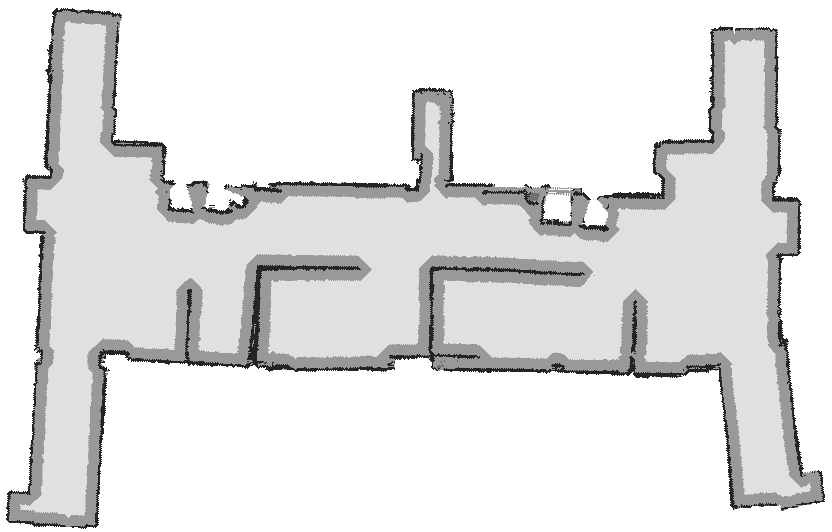
\includegraphics[width=\columnwidth]{inflated}
  \caption{Example of an inflated map used for PRM. Black pixels are obstacles. Grey pixels inside the map show the inflation applied to the obstacles.}
  \label{fig:inflatedmap}
\end{figure}
When checking the validity of points and lines on the map, it is necessary to take into account the size of the robot. This can be done by checking a radius around each point for obstacles, but for the purposes of efficiency, we have taken a slightly different approach. Instead of checking the area around points, we increase the size of obstacles by the required safe distance from obstacles. In our case, this is slightly above half of the longest dimension of the robot. After applying this size increase, we receive an ``inflated'' map, an example of which can be seen in Figure \ref{fig:inflatedmap}, which we use when generating the graph and for path planning.

When querying the PRM, a the robot's current position and the goal location are added to the graph and connected in the same way as other vertices. Dijkstra's algorithm is then run with the newly added vertices as parameters, and the shortest path between the vertices is returned. While using the raw path is viable, it can be further improved by smoothing. As seen in Algorithm \ref{alg:pathsmooth}, redundant intermediate vertices are removed from the path in an iterative fashion. $I$ is the number of smoothing passes executed, and $P$ is a vector of waypoints along the path. $P_n$ represents the $n$th waypoint in the path. The intermediate waypoint $b$ is removed only if there is a valid path between waypoints $a$ and $c$. The algorithm terminates either when the requested number of iterations has completed or if the path cannot be smoothed further. The benefit of smoothing is twofold; the path length becomes closer to the optimum, and the number of vertices in the path are reduced. The fewer vertices there are in the path, the less the robot must rotate during travel, and this results in a faster travel time from start to goal.

When a path has been found, a message is sent to a topic announcing that a path to the goal was found. In cases where a path cannot be found with the current graph that the PRM holds, the graph will be regenerated and searched again a number of times. If a path still cannot be found after the specified number of regenerations has occurred, the PRM will publish a message informing listening nodes of this fact so that they can handle the consequences.

\begin{algorithm}
  \caption{Path Smoothing}
  \label{alg:pathsmooth}
  \begin{algorithmic}[1]
    \State \textbf{Algorithm smooth\_path}\textnormal{($P, I, map$)}
    \For {$i = 0$ \textbf{to} $I$}
    \For {$j = 0$ \textbf{to} $\left|P\right|-2$}
    \State $a \gets P_i$
    \State $b \gets P_{i+1}$
    \State $c \gets P_{i+2}$
    \If{\textbf{vpath}$(map,a,c$)}
    \State \textbf{remove}($P,b$)
    \EndIf
    \EndFor
    \If{path not modified}
    \State break
    \EndIf
    \EndFor
    \State \textbf{return}\textnormal{ $P$}
  \end{algorithmic}
\end{algorithm}

\subsubsection{Navigation Node}
The navigation node moves the robot along paths provided by the PRM, and uses the estimated pose provided by the localisation node as the robot's current position. When a path is received, the first point is removed and set as the current waypoint to navigate to. The first action taken by the navigation node is to rotate towards the point until the robot heading and the bearing of the point from the robot's current location are within 0.15 radians of each other. With this constraint, we can be sure that the robot's heading is very close to the bearing of its destination before any movement is made towards it. If the waypoint is a particularly long distance away, the error between the heading and bearing at the starting location gradually increases as the robot nears the waypoint. If the error is below the 0.15 radian threshold, then only translational movement is applied, but if the error exceeds the threshold, angular movement is also applied, and the robot moves in a smooth curved path towards the waypoint. Adjusting for the error while moving means that the robot does not have to stop to adjust, which decreases the time spent travelling to the goal. Each waypoint has a radius of 0.2 metres, within which the robot is considered to have arrived at the point. When an intermediate waypoint is reached, the next point is removed from the path and set as the destination. The path is gradually consumed in this way until the goal is reached, at which point message is published informing any listening nodes of the fact.

The navigation also performs obstacle detection, by using laser data. An area of 90$^\circ$ directly in front of the robot is split into 10 sectors, from each of which a median distance reading is drawn. The median is used to reduce the effect of noise and erroneous readings. If the median of any sector is within a safe distance of 0.5 metres, a flag is raised and movement commands will no longer be sent to the motors. The position of the detected obstacle is calculated using trigonometry and placed onto a temporary map, which is passed into the PRM. The obstacle is detected as a point on the map, which is then inflated in the same way as the map used in the PRM. The PRM then prunes vertices which fall within the obstacle, as well as connections between vertices that pass through the obstacle. When this process is complete, the navigator re-sends the goal to the PRM which generates a new route, avoiding the obstacle. Obstacles are removed from the map when the robot is more than 4 metres from their location, or when it arrives at its goal. When an obstacle is removed, the graph is reconnected to ensure that the connectivity of the graph is not permanently affected.
\subsubsection{Vision Node}
For face detection, we decided to make use of camera data from the Kinect. Face detection in ROS necessitates the use of a vision library. We decided to use OpenCV as it is a highly popular tool in the research field, and is written in part by the ROS developers, suggesting easier integration. Communication between ROS and OpenCV requires the cv\_bridge stack, which is only compatible with C++ and Python. We decided that C++ was a better candidate than Python as face detection is very computationally expensive, and the C++ is a compiled language, which results in faster execution.
\begin{figure}
  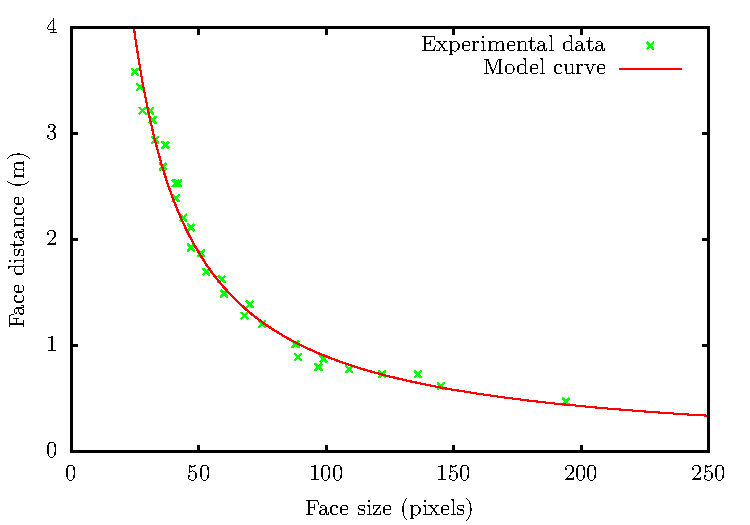
\includegraphics[width=\columnwidth]{centre_model}
  \caption{\textbf{MORE DETAIL}Depth model for the centre of the Kinect's field of view.}
  \label{fig:model}
\end{figure}
The OpenNI SDK publishes many ROS topics containing a variety of data from the Kinect. We made use of two of these topics, one providing depth and one RGB image data from the Kinect camera. These two topics are subscribed to by the C++ node that we created to allow the use of OpenCV with the Kinect image data. The output from OpenCV is then used in conjunction with the Kinect depth data to gain further confidence in whether a face has been detected. The C++ node publishes the location of the detected face along with the depth (i.e. distance to the face). This data is subscribed to by the control node which then uses the data accordingly.

The face detection system using OpenCV worked as expected, but gave many false positives, detecting cabinets and clothing as faces, even after we tuned the parameters that were available to us. We decided to use the Kinect's depth information to decide which detections were actually faces. To do this, we considered the fact that many of the false positives were much larger or much smaller than actual human faces, and that human faces do not tend to vary much in size. Using the size of the rectangle representing the potential face in the image along with the depth of the potential face, we can determine whether the rectangle is a real face by comparing it against the expected depth and rectangle size. To obtain these values, we created a face size model by recording measurements of real faces. We had two human participants, one tall and one short, stand 0.3m from the camera and take small steps backwards until they were 3.5m away, as we recorded the measurements of depth and rectangle size. Once we had these values, we plotted them on a graph and programmatically found a quadratic line of best fit, shown in Figure \ref{fig:model}. The line of best fit is our model, which we can use to compute an expected value for either depth or face size, as long as we have the other. Once this model was included in the node, rectangle sizes from detections were used to determine expected depth and compared with the depth data from the Kinect. When they were not within a set tolerance, the detections were discarded as false positives.

\begin{algorithm}
  \caption{Face detection}
  \label{alg:facedetect}
  \begin{algorithmic}[1]
    \State \textbf{Algorithm detect\_face}\textnormal{(image)}
    \State face\_rects$\leftarrow$\textbf{haarDetect}(image, haar\_cascade)
    \For{face in face\_rects}
    \If{$\neg$\textbf{validFace}(face, depth)}
    \State \textbf{remove}(face\_rects, face)
    \EndIf
    \EndFor
    \State \textbf{publish} face\_rects
  \end{algorithmic}
\end{algorithm}
Algorithm \ref{alg:facedetect} shows our face detection algorithm. In line 1, a Haar feature detector is run on the image received from the Kinect video feed, from which a series of rectangles representing possible faces are received. Non-faces are removed from the array in line 4. If valid faces remain after the array has been checked, they are published to the network. Face validity is determined by Algorithm \ref{alg:faceprune}. In line 2, depth values from a smaller rectangle of 20\% width and height of the original rectangle, in the centre of the original rectangle are retrieved. We use the median depth of this smaller area as the actual depth of the potential face. If the median of the area exceeds a threshold of 3.5m as per the effective range of the face detection algorithm, the face is rejected. Otherwise, in lines 7--10, the expected depth and actual depth are compared. The tolerance value $\alpha$, set to 15\%, is applied to the value expected by the model. If the actual depth is within this tolerance range, the face is considered valid.
\begin{algorithm}
  \caption{Face validity check}
  \label{alg:faceprune}
  \begin{algorithmic}[1]
    \State \textbf{Algorithm validFace}\textnormal{(face\_rect, depth)}
    \State depth\_pixels$\leftarrow$\textbf{getCentreRegion}(face\_rect)
    \State median$\leftarrow$\textbf{getMedian}(depth\_pixels)
    \If{median$>$threshold}
    \State \textbf{return} False
    \Else
    \State expected$\leftarrow$\textbf{expectedDepth}(face\_rect)
    \State tolerance$\leftarrow \alpha \cdot$expected
    \State diff$\leftarrow \left|\textnormal{median}-\textnormal{expected}\right|$
    \If{diff$>$tolerance}
    \State \textbf{return} False
    \EndIf
    \EndIf
    \State \textbf{return} True
  \end{algorithmic}
\end{algorithm}

With our first implementation of this model, referred to as depth model 1, we noticed that the expected depth values were causing the model to discard valid faces in the far left and far right of the field of view of the camera. Although the Kinect sensor manufacturer claims to adjust for angle distortion, it is clear that there is some discrepancy at larger angles. We found that the model worked well for the central 40\% of the image (roughly 95\% true positive rate), while there was a smaller true positive rate for the left and right 30\% of the image (roughly 60\%). This led us to create a pair of models, one for the centre of the image, one for the left and right hand sides, to replace the previous model. We created these in the same way as the previous model. For each model (centre and angle), we collected data for two participants of varying height and combined them. The models are used conditionally---if the centre of the face rectangle is within the central 40\% of the image, the centre model is used, otherwise the angle model is used.

\subsubsection{Control Node}
\label{sec:control}
The control node can be thought of as a finite state machine, where there are several states in which the machine can be, and it transitions between these states until it reaches the completed state. A simplified diagram can be seen in Figure \ref{fig:fsm}. The robot starts in the \emph{initialisation} state, and waits to receive a map of the space that it is to work in. Once a map has been received and pose estimates are being received from the localisation node, the robot moves into the \emph{finding room} state, in which it attempts to locate an empty room that it can take people to. Due to time constraints, the central points and bounding boxes of the two meeting rooms available on our map were hard coded into the system. The robot uses the PRM to navigate to the meeting room closest to its current location, and once inside, performs a 360$^\circ$ scan of the room to check whether it can identify any faces. When a message is received from the vision node containing rectangles representing faces in the field of view, the robot transitions into the \emph{face check} state. In this state, the robot attempts to confirm whether what is being seen is actually a face or not. A face is confirmed when the vision node sends three successive messages which all contain a face in the same area. When the first message is received, the rectangle with the lowest depth value is selected. When subsequent messages are received, the rectangle with the centre closest to the previous rectangle is selected, and a check is made to see if this rectangle's centre is within the bounds of the previous rectangle. If one of the subsequent messages contains no rectangles, or contains rectangles which are too far from the previous rectangle received, the robot returns to scanning the room. If a face is confirmed, the room is occupied and the robot moves to the next room and performs the same scan. If the second room is also occupied, it will return to the first room and check again. This will be repeated until an empty room is found.
\begin{figure}
  \centering
  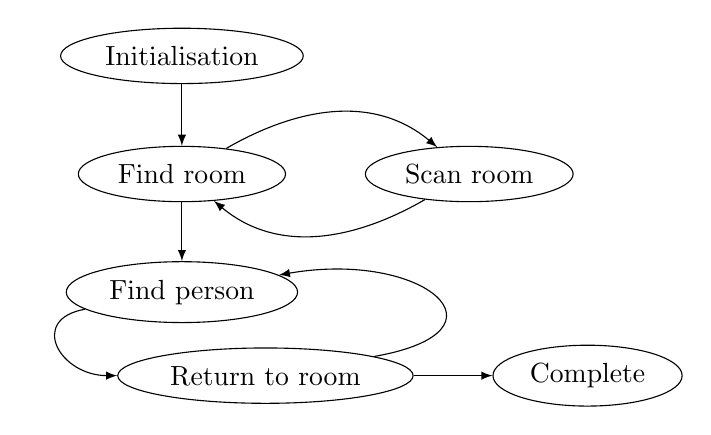
\begin{tikzpicture}
    \node [cloud] (init) {Initialisation};
    \node [cloud,below of=init] (findroom) {Find room};
    \node [cloud,right=1cm of findroom] (scan) {Scan room};
    \node [cloud,below of=findroom] (findp) {Find person};
    \node [cloud,below right of=findp] (return) {Return to room};
    \node [cloud,right=1cm of return] (comp) {Complete};
    \draw [->] (init)--(findroom);
    \draw [->] (findroom) to [out = 30, in = 140, looseness = 1] (scan);
    \draw [->] (scan) to [out = 210, in = 320, looseness = 1] (findroom);
    \draw [->] (findroom)--(findp);
    \draw [->] (findp) to [out = 190, in = 180, looseness = 2] (return);
    \draw [->] (return) to [out = 10, in = 10, looseness = 3] (findp);
    \draw [->] (return)--(comp);
  \end{tikzpicture}
  \caption{Simplified version of the finite state machine used in the control node.}
  \label{fig:fsm}
\end{figure}

Once an empty room is found, the \emph{exploring} state is entered. To save time, we decided to adapt the sampling methods used for PRM to generate exploration paths. Using cell sampling, one point is sampled in each cell with a width of four metres. Points are not sampled within meeting rooms, as we are only concerned with people outside the meeting rooms. The current robot location is connected to the point closest to the robot, and that point is connected to the closest point to itself. Subsequent points are connected in the same way until a single path is constructed. The first point in this path is set as the goal location, and the robot moves to it using the PRM. Once the point has been reached, the next point is consumed, and so on until the end of the exploration path is reached. When this happens, points are once again sampled, but this time with a cell width of two metres. When the path generated from this is consumed, the cell size is set to one metre. After that, the cell size is once again set to four metres and the cycle continues. Decreasing the cell size means that more points are sampled into the map, and so places which may not have been explored with a larger cell size have a chance of being visited. If a face is seen while the robot is exploring, the robot will attempt to centre the face in its field of view and then confirm that it is a face in the same way as described above. If a face is confirmed, then the robot will set a goal to just in front of the expected location of the person calculated from the depth of the rectangle. When the goal is reached, a sound is played to alert the person, who is asked whether they would like to attend the meeting via a dialogue box. If the person accepts the invitation, the robot guides the person back to the meeting room that it found was free in the finding room state. We assume that the person follows the robot once the invitation is accepted. If the invitation is declined or a 15 second timer expires, the robot continues exploring. The robot is provided with a number of persons that it must find and bring to the meeting room, and once that number of persons have been found and brought to the room, the task is complete and the system is shut down.

\textbf{Any more assumptions?}We make several assumptions about how the world works. Due to limitations with our face detection, persons who we are trying to find are assumed to be facing the robot at all times. We also assume that the person follows the robot to the meeting room, and that people who have been taken to the meeting room do not leave.

\section{Experimentation}
In this section we display the results of experiments carried out to determine the best algorithms, parameters or strategies to use in various parts of our system.
\subsection{MCL Tracking Error}
\begin{figure}
  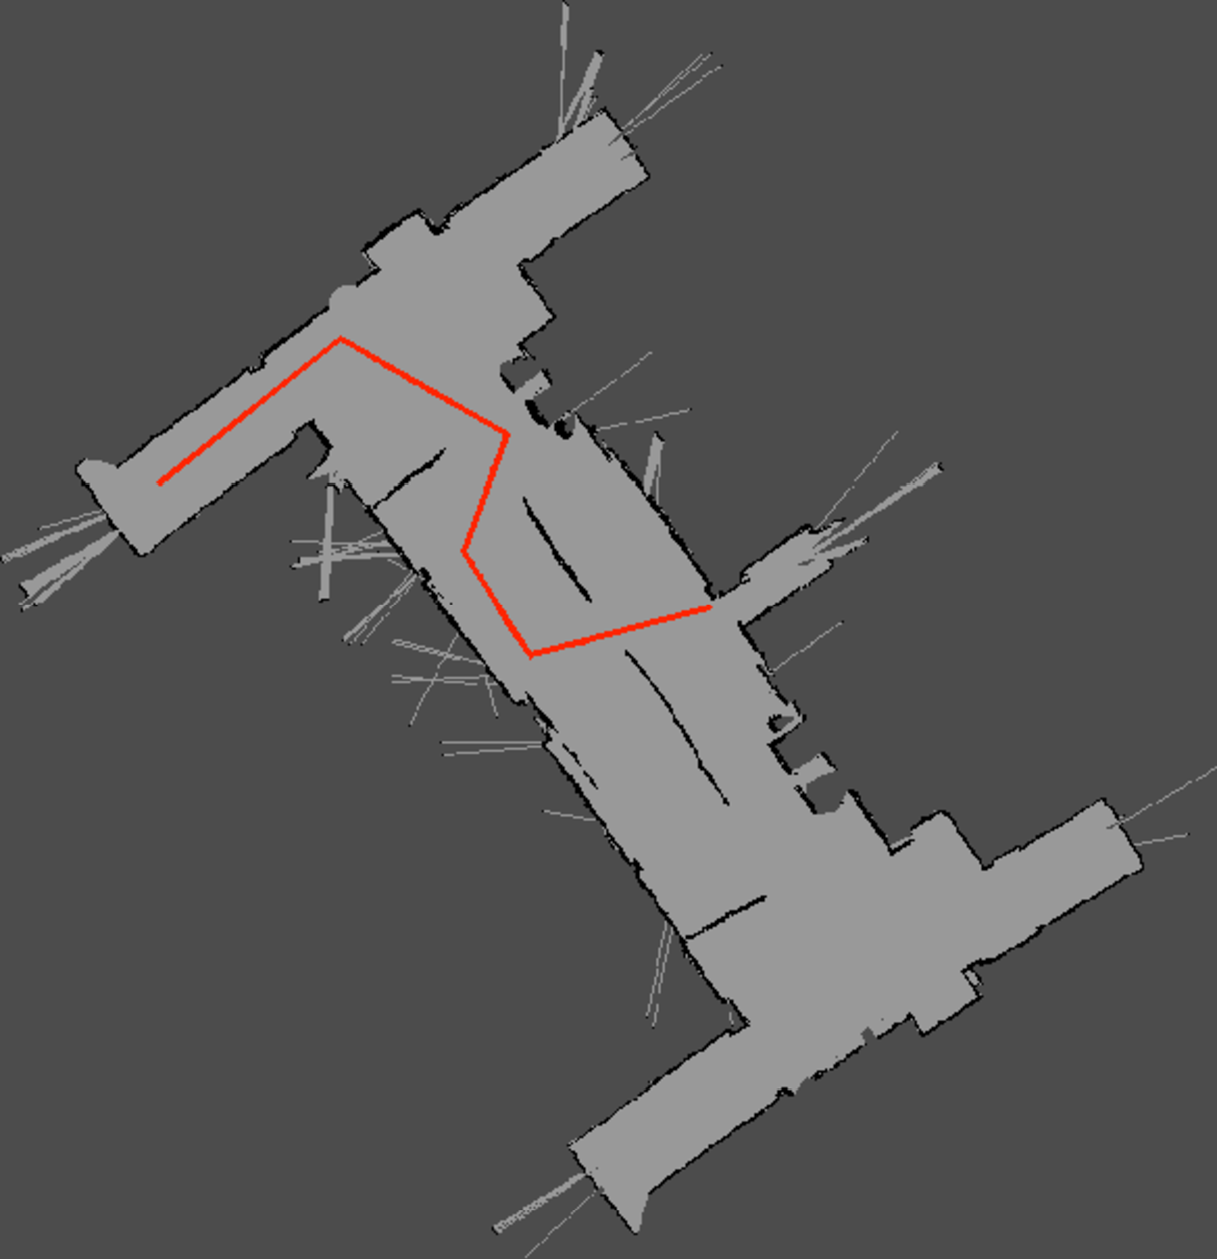
\includegraphics[width=\columnwidth]{localisation-experiment-path}
  \caption{Path used for tracking error experiment.}
  \label{fig:locpath}
\end{figure}
\subsubsection{Aim}
The aim of this experiment is to compare the tracking error of three different MCL implementations; the built in ROS AMCL and two of our own implementations.
\subsubsection{Method}
As each MCL implementation has many different variables, we will use the set of variables that resulted in the best performance in past experiments. To provide accurate results, we require a ground truth, which will be obtained from the Stage simulator. We will run the experiment three times for each implementation and record the tracking error every second while the robot moves, until it reaches the end of its path. The tracking error is defined as the Euclidean distance between the ground truth and the estimated pose provided by the localisation at each point at which a measurement is taken. The robot will start from the same initial position and follow the same path, seen in Figure \ref{fig:locpath}, in each experiment.
\subsubsection{Results}
Figure \ref{fig:local} shows the tracking errors for each implementation, with error bars representing the standard deviation over three runs. Apart from two anomalous points at 13 and 25 seconds at which all implementations experience an increase in tracking error, the deviation of AMCL is significantly lower than the other two implementations. The average deviation over the three runs for AMCL is 0.019m, compared to averages of 0.071m and 0.085m for Penny and Leslie respectively. It is clear that to obtain accurate position estimates we should make use of ROS AMCL.
\begin{figure}
  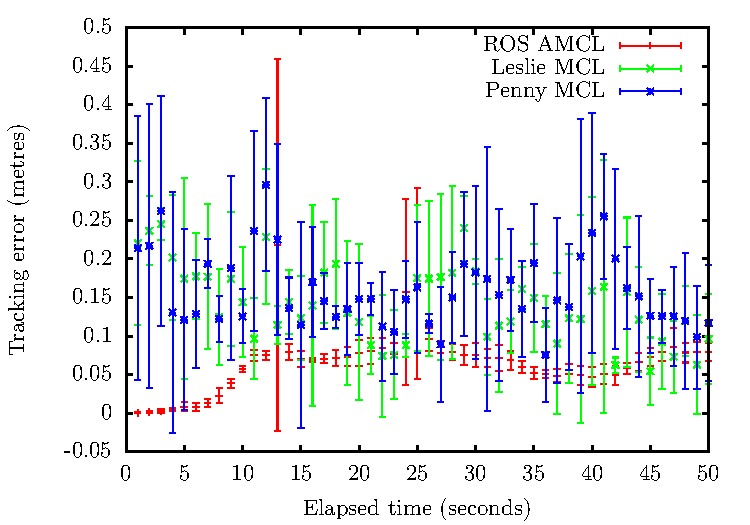
\includegraphics[width=\columnwidth]{tracking_stdev}
  \caption{Comparison of Tracking error of ROS AMCL and two independently developed MCL algorithms}
  \label{fig:local}
\end{figure}
\subsection{PRM sampling methods and connection strategies}

\subsubsection{Aim}
The aim of this experiment is to find the sampling method and connection strategy which, as a pair, produce the shortest path lengths on average.
\subsubsection{Method}
To find the best sampling method and connection strategy pair, we created four qualitatively different pairs of start and end points. We passed each point pair to the PRM, applied the path smoothing algorithm to the generated path and measured its length. We varied the maximum number of connections per node---using values of 5, 10, 20 and 30---\textbf{i don't really get this}and only chose the best path length value since this value has a large effect on the path length depending on the sampling method and connection strategy chosen. In addition, we experimented with different values for variables specific to each sampling method. For grid sampling we varied the size of the x and y step, using values of 0.5m, 1m, 2m and 4m. For cell sampling we varied the number of points sampled in each cell, either 2 or 5, and used 1m, 2m, 4m and 6m cell sizes. For random sampling, we varied the total number of points sampled, using values of 25, 50, 100, 200, 400 and 800. We ran three trials for every combination of sampling method, connection strategy, maximum connections per node, and pair of start and end points as well as every combination of variables specific to each sampling method.

We chose four start and end point pairs which would provide qualitatively different paths, allowing us to compare the various techniques in different environments, ensuring we choose a combination which is able to generalise well. Point pairs were chosen to give examples of long, medium and short paths through the map. Finally, we added a pair in which the goal point is within a narrow corridor. This final pair should give us data about how well the sampling method deals with difficult areas of the map.
\subsubsection{Results}
The experiment produced four path length values for every combination mentioned above, one for each pair of start and end points. Sets of four values cannot be compared at once, so in order to compare combinations, these four path lengths must be combined into a score which indicates how good the paths are. To create such a score, we determined the theoretical optimum path length by manually tracing lines on the map and measuring their length. These are the lines shown in Figure \ref{fig:optimum}. The score for a combination of variables and methods is calculated as the ratio between the computed path length and the theoretical optimum. For example, if the minimum length were 10m and the computed length were 12m, the ratio as a decimal number is 1.2. To achieve a combined score for all four paths, we average the four scores. Figure \ref{fig:sampleconntable} shows the best scores achieved by sampling method and connection strategy combinations.

\begin{figure}
  \centering
  \begin{tabular}{|c|c|c|}
    \cline{1-3}
    Sampling Method & Connection Strategy & Best Score      \\ \cline{1-3}
    \multirow{3}{*}{Cell} & Neighbourhood & \textbf{\textcolor{red}{1.03909}}         \\ \cline{2-3}
    & NearestN  & 1.09907                                     \\ \cline{2-3}
    & Threshold & 1.12969                                       \\ \cline{1-3}
    \multirow{3}{*}{Grid} & Neighbourhood & \textbf{1.03693}                          \\ \cline{2-3}
    & NearestN & 1.14463                                        \\ \cline{2-3}
    & Threshold & 1.05153                                       \\ \cline{1-3}
    \multirow{3}{*}{Random} & Neighbourhood & \textbf{1.02578}                        \\ \cline{2-3}
    & NearestN & 1.05171                                      \\ \cline{2-3}
    & Threshold & 1.06639                                     \\ \cline{1-3}
 \end{tabular}
  \caption{\textbf{maybe a little unclear?}Best scores for each combination of sampling method and connection strategy}
  \label{fig:sampleconntable}
\end{figure}

The best score (lower values are better) is achieved by random sampling with the neighbourhood connection strategy. However, during the experiment the trials for this combination did not always compute a path. In particular, a path could not be computed where the end point was within the narrow corridor. This is due to the fact that with random sampling nodes are randomly distributed across the map with no regard for the fact that narrow areas have a smaller probability of having nodes generated within them. This means that often, there are no nodes generated within the corridor and thus no path can be computed. Since this combination could not compute a path in one of our test cases, we cannot use it.

The next best score achieved was by grid sampling and the neighbourhood connection strategy. This combination, similarly, consistently could not compute a path to the end point within the narrow corridor. This is easily explained by the nature of grid sampling; the nodes are placed across the map as evenly spaced points, but those which coincide with walls or non-map space are discarded. This means that narrow areas have a small probability of having nodes placed within them. Again, we cannot use this combination because it does not compute a path in our test scenario.
\begin{figure}
  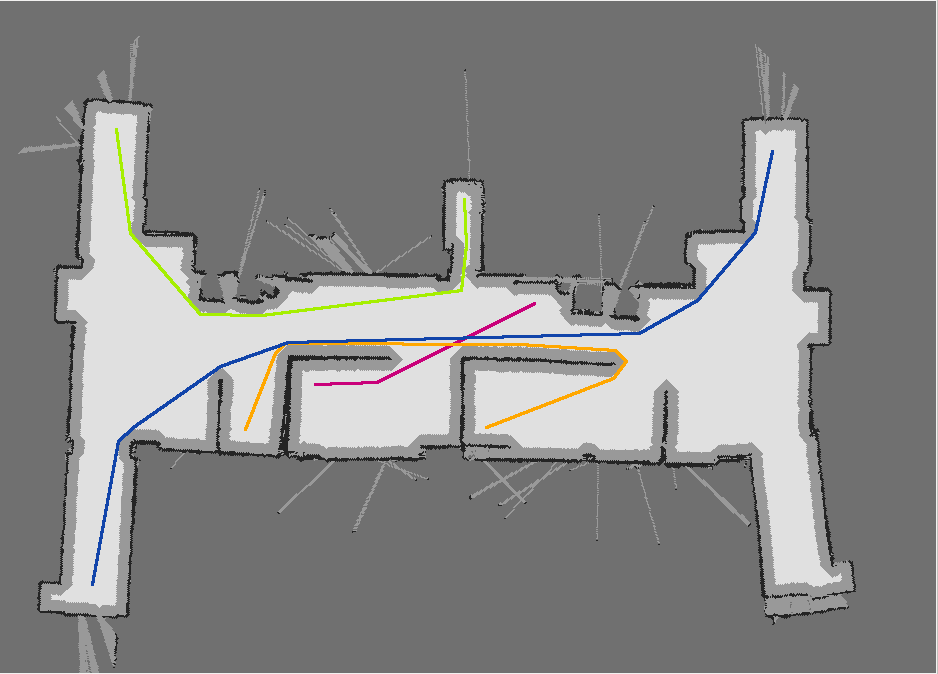
\includegraphics[width=\columnwidth]{optimumpaths}
  \caption{Optimum paths used for comparison of connection strategies and sampling methods.}
  \label{fig:optimum}
\end{figure}
The third best score was achieved by cell sampling and the neighbourhood connection strategy. This combination was consistently able to compute paths in all cases in the experiment. The reason is fairly clear; cell sampling is designed to ensure complete coverage of the free space in the map and provides a higher probability of node coverage in narrow areas containing walls or non-free space. We could not see any qualitative objections to using this combination, so this is chosen as the best combination. Specifically, this combination used 30 maximum connections per cell, a cell width of 1m and a target number of nodes per cell of 5.


\subsection{Haar cascade efficacy}
\begin{figure}
  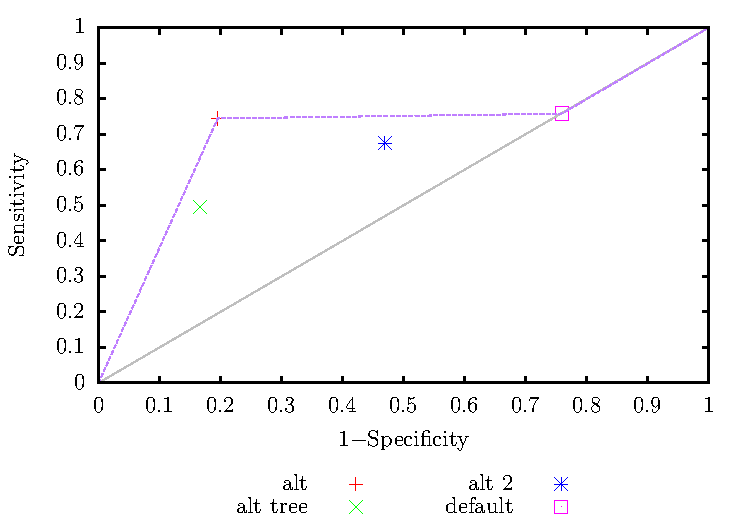
\includegraphics[width=\columnwidth]{haar_ROC}
  \caption{ROC graph of frontalface Haar cascade results.}
  \label{fig:haar}
\end{figure}
\subsubsection{Aim}
The aim of this experiment is to find the Haar cascade most suited to perform face detection with the Kinect. We wish to find the cascade which has the highest specificity and sensitivity; all actual faces should be classified as faces, and anything which is not a face should be ignored.
\subsubsection{Method}
To test the different Haar cascades we captured a set of images using the Kinect camera which all included faces in different surroundings and at different angles. We then processed each image using our cascade-based face detection node which works on still images, using the frontalface\_default, frontalface\_alt, frontalface\_alt2 and frontalface\_alt\_tree cascades. We manually analysed the processed images, which contain rectangles indicating the areas detected as faces. In order to generate the data, we looked at the image output from the program for each cascade and analysed the number of faces that were correctly detected (true positives), the number of non faces not detected (true negatives), the number of falsely detected faces (false positives) and finally, the number of faces which were completely missed (false negatives). Once we had all these values for each image, we averaged the sensitivity for each Haar cascade to find their final value.
\subsubsection{Results}
From our results of the above experimentation it was obvious that none of the cascades performed well on profile faces. This was expected as the cascades we used were specifically trained on frontal face images. The default and alt cascades performed better on faces at an angle than the alt2 and alt tree. The alt and default cascades also performed well on frontal face images with various backgrounds. As is obvious from the ROC graph in Figure \ref{fig:haar}, the best performer was the alt cascade. Although its sensitivity value of 0.744 was slightly  lower than the 0.758 of default, the alt cascade performed a lot more effectively detecting true negatives (i.e. correctly identifying no faces exist). This result pushed the $1-$specificity reading for the alt cascade towards the left, highlighting it as the best candidate. Although the default cascade performed better in the sensitivity reading, it also performed worst in the 1-specificity reading, frequently classifying non faces as faces. It is clear that cascade which performed best was frontalface\_alt, classifying actual faces as faces with a good degree of consistency. As the cascade still detected false positives, we decided attempt to reduce the frequency of these by combining depth information from the Kinect with a model of face size.
\subsection{Adding the Kinect depth model}
\subsubsection{Aim}
The previous experiment established the best Haar cascade to use in our vision node. However, there are assumptions we can make which were not made in the last experiment. The aim of this experiment is to determine the performance of face detection when making some assumptions about the world, as well as using a face size model.
\subsubsection{Method}
Since we are trying to improve detections for this cascade with our face size model, we performed this experiment in the areas where all the cascades generally performed badly (had many false positives). In this area, we used all of the cascades to find features of the scene which were falsely detected as faces. We noted these for reference as 'true negatives' which we can eliminate with our new depth model. To determine the sensitivity and specificity of the vision node with the new assumptions, both before and after the inclusion of both Kinect depth models (depth model 1 and depth model 2 as described in the Design section), we designed a single experiment which would produce results for all three at once.

We modified our vision node to show rectangles of different colours based on whether they would be accepted by model 1 or model 2. We had a participant move within the depth of field of the camera to 100 different positions and we took readings for true and false positives and negatives. Alongside the features of the scene we noted earlier which we hoped to eliminate as true negatives, this allows us to gain three points on the ROC graph to compare.
\subsubsection{Results}
The resulting ROC graph is shown in Figure \ref{fig:cascade_with_model}. The point labelled 'alt (no assumption)' is the point taken from the last experiment. We collected 11 scene features which were falsely identified by the cascades as faces. This means that the 1-specificity axis of the ROC graph is of a fairly low resolution. However, with 100 true faces, the sensitivity axis is of a high resolution.

We can see in the graph that sensitivity and the 1-specificity value have both increased. It appears that adding the assumption of faces being directed towards the camera increases sensitivity, while performing the experiment within an area where cascades tend to perform badly causes the 1-specificity value to increase.

Using depth model 1 we see that we have decreased both the sensitivity and the 1-specificity value. The decrease in sensitivity is clearly due to the wrongful discarding of real faces done by model 1 on the left and right hand sides of the image. However, the correct discarding of false positives have also decreased the 1-specificity value. Overall, this point is better in some respects and worse in others when compared with using no model at all.

When using depth model 2, we see that the performance improves greatly. This depth model discards none of the true positives given by the cascade, keeping its sensitivity identical to using no model at all. However, false positives are down to 0, making the 1-specificity value also 0. It is worth noting that, since there were only 11 'true negatives' being sought, this value being 0 may be slightly misleading and may well be higher with a larger number of true negatives. Using depth model 2 cannot improve on the sensitivity of using no model at all, but by eliminating all true negatives it is clearly the best point on the ROC graph and is certainly worth using.

\begin{figure}
  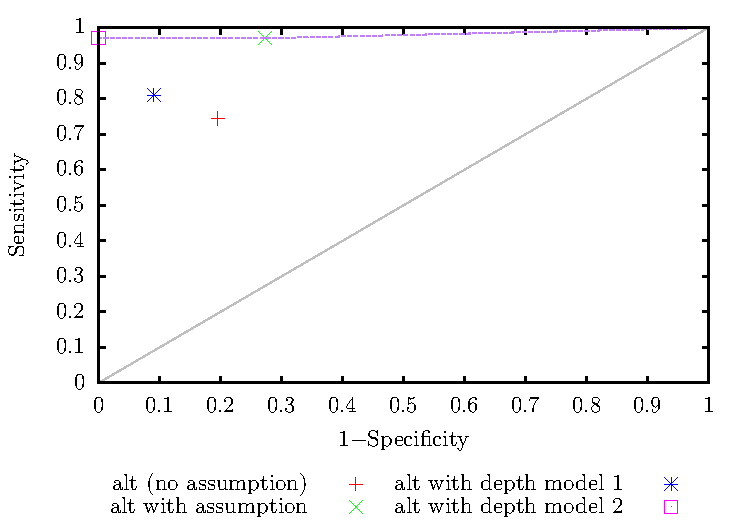
\includegraphics[width=\columnwidth]{kinect_ROC}
  \caption{ROC graph of frontal\_face\_alt cascade performance with assumption that subjects face the camera and with depth models applied.}
  \label{fig:cascade_with_model}
\end{figure}
\subsection{Exploration coverage}
\subsubsection{Aim}
In this experiment, we aim to find the best method of sampling points on the map so that the robot can explore most space in the shortest amount of time.
\subsubsection{Method}
We let the robot explore the map in simulation, as described in Section \ref{sec:control}, for 8 minutes, using each of the sampling methods with four different strategies (8m-6m-4m, 6m-4m-2m, 4m-2m-1m and 2m-1m). We used ray tracing to project the field of view of the robot onto an occupancy grid. Each grid cell the ray passed through was counted as explored. Rays originated 0.3m in front of the robot and travelled outwards until the ray was obstructed by a wall or reached the maximum effective distance of the face detection node of 3.5m. The number of free cells remaining in the map was calculated each second. As we do not explore the meeting rooms, cells inside these areas were not counted in the total. Each experiment will be run for 8 minutes. The movement speed of the robot affects the speed of exploration. The maximum movement speed and rotation speed were set to 0.7m/s and 0.4rad/sec respectively in each experiment.

\subsubsection{Results}
As can be seen in Figure \ref{fig:covtbl}, the cell based exploration consistently covered more of the map than the grid strategy. Figure \ref{fig:coverage} shows the best run of the best strategy for each method. After 300 seconds, the grid method stopped covering new areas of the map, while the cell based method continued to increase its coverage. The effectiveness of the exploration can also be shown as a heat map. Figure \ref{fig:heatmap} shows the heat map at the end of the best cell method run, which shows that almost the whole map was explored, with relatively even coverage.
\begin{figure}
  \centering
  \begin{tabular}{|c|c|c|}
    \cline{1-3}
\multirow{2}{*}{Strategy}& \multicolumn{2}{ c| }{Sampling method} \\ \cline{2-3}
& \multicolumn{1}{c|}{Cell} & \multicolumn{1}{c|}{Grid} \\ \cline{1-3}
\multicolumn{1}{ |l| }{2m$\rightarrow$1m} & 91.3 & \textbf{89.4}      \\ \cline{1-3}
\multicolumn{1}{ |l| }{4m$\rightarrow$2m$\rightarrow$1m} & \textbf{94.0} & 86.4  \\ \cline{1-3}
\multicolumn{1}{ |l| }{6m$\rightarrow$4m$\rightarrow$2m} & 93.5 & 83.5  \\ \cline{1-3}
\multicolumn{1}{ |l| }{8m$\rightarrow$6m$\rightarrow$4m} & 93.7 & 82.8 \\ \cline{1-3}
  \end{tabular}
  \caption{Percentage coverage after eight minutes of exploration with different strategies and sampling methods.}
  \label{fig:covtbl}
\end{figure}
\begin{figure}
  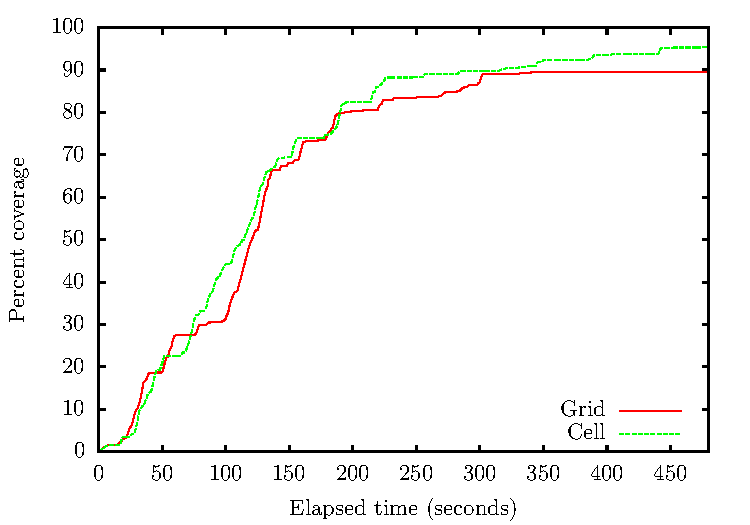
\includegraphics[width=\columnwidth]{percent_coverage_time}
  \caption{\textbf{REWRITE}Comparison of the best grid and cell based exploration strategies. The heatmap corresponding to the cell run is found in Figure \ref{fig:heatmap}.}
  \label{fig:coverage}
\end{figure}

\begin{figure}
  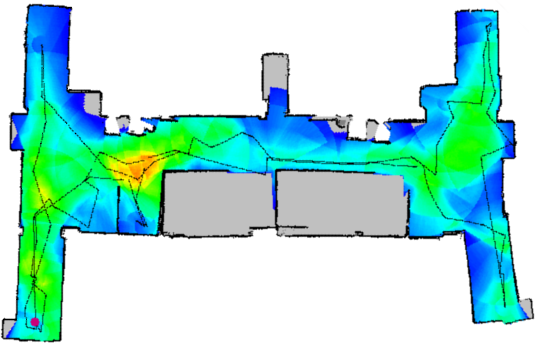
\includegraphics[width=\columnwidth]{4-1_1}
  \caption{Heat map showing coverage over an 8 minute run using the best cell based strategy. The colour gradient goes from red (high) to blue (low). The pink dot shows the starting location. The black line is the path taken by the robot.}
  \label{fig:heatmap}
\end{figure}

\subsection{Meeting room availability confirmation}

\subsubsection{Aim}
The aim of this experiment is to test how well our robot performs in finding an empty room. We wish to test the robots ability to handle different events during the meeting room availability confirmation stage.
\subsubsection{Method}
To test the robots performance in finding an empty room, we derived three events which are likely to occur and therefore have an effect on the robots performance during the task. The first event is the event in which the first meeting room the robot PRMs to was empty. The second event which was presented to the robot, was the event in which the first meeting room was not empty, however the second meeting room was empty. The third and final event tested was the event in which both the meeting rooms were occupied. In order to test these different events we had to ensure we placed the robot in particular locations in order to test the robots ability to check its nearest meeting room first. Therefore we had two starting position for the robot in order to perform the experiment in which both meeting rooms could be picked first. These positions were the same corner of the map however on opposite sides of the map. In order to record the results of this experiment, we timed how long the robot took in each of the three different scenarios from both starting positions on the map.
\subsubsection{Results}
The result of this experiment indicates that our robots ability to find an empty room or continue to check for a meeting room in the case of no empty meeting room completes in a sufficient time. In a worst case scenario where an exhaustive search is performed, i.e. both meeting rooms are occupied, the robot took 2:17 on average (averaged from the result of the runs from the two different starting locations) to confirm there are no empty rooms and to continue searching. Otherwise if the first meeting room was empty, the robot took 1:25 which is a reasonably quick time for a room to be confirmed empty. Finally if the first meeting room was classified not empty and the second was empty, the robot took 2:22 on average, which again is a reasonable time. The reason the average time for the exhaustive search from the different locations is slightly quicker in comparison to the event with only one meeting room free is most likely due to PRM as the path which it took may have been different and longer. We saw that the robot successfully identified the nearest room correctly each time it was run from the two different locations. We also observed the robot successfully plan routes to the centre of rooms and also routes between the two rooms in order to check them. Overall due to the small amount of time taken to perform the three tests provided, we believe the robot performed consistently well.
\subsection{Gathering meeting attendees}

\subsubsection{Aim}
The aim of this experiment is to test the robots ability to gather meeting attendees. This experiment in combination with the previous experiment are the most important as they allow us to analyse the robots performance within the whole task.
\subsubsection{Method}
In order to test the robots performance in this specific task, we generated three possible environments in which we tested an extreme case and more likely cases. In order to test the extreme case, we decided to place an attendee at a large distance from the room, and then another attendee at a large distance from the first attendee. For one of the other two cases, we placed attendees very close to the meeting room to record the robots performance in finding attendees who were very close to the door of the meeting room. For the final case, we decided to place an attendee at half the distance of the maximum distance found from the meeting room in case one, and the second person at the same distance from the other attendee. The justification for the second attendee to be placed at such distances from the first attendee was in order to be able to test the exploration. Exploration continues from the point where it found the attendee, and therefore after an attendee has been taken to the meeting room, exploration will begin from that point. In order to gather results, we ran this experiment enough times in order to be able to get 2 successful runs without human intervention, which we could then average. We recorded the average time of the experiment, the number of times it missed attendees during successful runs and finally the number of failed attempts which are classified by experiments which required human intervention. The total time which is available for the full task is 15 minutes, therefore in order to assess the robots ability to complete the full task successfully, the combined time from the previous experiment for finding a room and this experiment should total to less than 15 minutes.
\subsubsection{Results}
\label{sec:attendres}
From the results table  in Figure \ref{fig:fullsystem} we can observe that the time taken to find the attendees was rather reasonable. If we look at the worst case scenario time of 11:55 on average, we can see that adding 2:22 to this time (longest time from the previous experiment) we are still within the 15-minute time limit. So in terms of efficiency we can deduce that the robot performed rather well as even in its worst case scenario it managed to perform the task within the time limit. However what we did notice on the experiments was the robot sometimes missed people who were in view and therefore did not PRM to them. The possible justification for this is that there were not enough frames (3 frames required to confirm face is true) for the robot to confirm the faces and therefore explaining why it missed the person. We saw this issue with all of our successful runs and the results of how often the attendees were missed on average can be seen in  Figure \ref{fig:fullsystem}. During the experiment we had many issues in regards to AMCL localising in an incorrect position, which caused it to collide with walls and objects and required us to intervene. This continuously required us to have to repeat the experiment in order to get a full run without human intervention. The reason for AMCL to lose its position frequently could be as a result of the map in real world being slightly different to the map provided. However taking this into consideration, we believe the whole system performed rather well as it correctly found empty meeting rooms and from there it managed to explore and correctly find attendees, occasionally missing some, however they were picked up soon again when the robot returned to explore in that area. We also observed that the exploration worked rather well too as even in the most extreme cases where attendees are standing in far corners, the robot managed to explore the area near them, identify and guide attendees to the meeting room.
\begin{figure}
  \centering
    \begin{tabular}{r|r|r|r|}
    \cline{2-4}
    &Short&Medium&Long\\\hline
    \multicolumn{1}{|r|}{Average time}&4:24&9:19&11:55\\\hline
    \multicolumn{1}{|r|}{Failed attempts}&4&5&10\\\hline
    \multicolumn{1}{|r|}{Missed persons}&1.5&4&5.5\\\hline
  \end{tabular}
  % \begin{tabular}{c|c|c|c|}
  %   \cline{2-4}
  %   &Average Time&Missed People (Avg)&Failed Attempts\\\hline
  %    \multicolumn{1}{|l|}{Short}&04:24&1.5&4\\\hline
  %    \multicolumn{1}{|l|}{Medium}&09:19&4&5\\\hline
  %    \multicolumn{1}{|l|}{Long}&11:55&5.5&10\\\hline
  % \end{tabular}
  \caption{THIS IS NOT A CAPTION}
  \label{fig:fullsystem}
\end{figure}

\section{Discussion}
Once our experiments provided the optimal configuration for the variables in our system, our full system tests showed that the robot completed the task within the 15-minute time limit even in our worst case scenario. The robot stayed within the task specification, finding empty rooms and attendees and taking attendees to the meeting rooms. However, the task was not always completed because the robot sometimes collided with walls and other objects. This was mainly due to issues with AMCL, as discussed in Section \ref{sec:attendres}.

When implementing individual components of the system, we found that the ROS publisher/subscriber model was sometimes helpful while at other times a hindrance. For example, this structure helped when developing the vision node since the main system was written in Java while the vision node was written in C++. Using the standard ROS architecture, there was minimal complexity in passing data from the C++ node to the Java node, whereas usually this is more complex.

We found during our implementation that generating intelligent behaviour in a robot is more difficult than it first seemed. This is due in part to the fact that the environment is non-deterministic and dynamic, and the sensors used to gather data are prone to noise. Furthermore, there are a very large number of scenarios---some of which seem obvious or trivial at first---that need to be considered during both design and experimentation, to increase the system's reliability and performance. For example, although we designed our system to avoid obstacles and plan around them, in the real world environment, obstacles which were detected, such as humans, would often disappear later and this had to be accounted for. To people unfamiliar with the field, the system that we have implemented would most likely appear decidedly \emph{unintelligent}, due to its limited capabilities

While the individual components and techniques we used in our robot were chosen using sound experimental analysis, there were some drawbacks to using them. Using AMCL for localisation rather than our own localisation implementation was the conclusion we came to after experimentation. However, since we did not implement AMCL ourselves, we could not find or correct issues with it when they occurred. By using our own PRM implementation we had the advantage of full control over the code, as well as full understanding of how it worked. On the other hand, the obstacle avoidance part of the navigation code needed improvement and due to time constraints we could not perform this improvement. This had a negative effect on our system's overall performance and was responsible for failed runs in some of our experiments. Using OpenCV for face detection worked well, but caused some problems. Firstly, processing images from the Kinect's camera was very slow, typically taking 300-400ms to detect faces using a single cascade in a single image. This meant that when the robot was moving, the face's detected position would vary greatly between detections. Another issue was the high rate of false positives for all of the Haar cascades. However, these issues did not prevent us from creating a highly successful vision node when coupled with the Kinect's depth data. Using the Kinect vastly improved our vision node and was easy to set up and use. The main issue with the Kinect was the low resolution of the camera, but our vision node did not suffer from this.

\subsection{Potential Improvements}
Although the vast majority of bugs were fixed, we were unable to determine the root of some issues which occasionally caused the system to crash. For a robot to be truly autonomous, it should have sufficient error handling capability to prevent minor issues causing the system to stop. Improvements could be made to the exploration path generation by using heuristics. The current method occasionally generates paths which are inefficient, requiring a lot of rotation, which slows down the exploration. A more advanced sampling method such as medial axis sampling could be used in the PRM in order to generate paths which are less likely to result in collisions. To further decrease time taken to gather attendees, any person seen while returning to the meeting room could be noted, and instead of resuming exploration, locations where people might be could be checked first. The use of multiple robots could further increase the efficiency of both exploration and attendee collection, although this would increase the complexity of the system. Improved human-robot interaction is also something that could be considered. Rather than using noises, communicating using natural language would give the humans the robot is interacting with more information about what it is doing.
\subsection{Conclusion}
In this report we have presented our system which, given a map and meeting room locations, locates an empty meeting room, finds people in the vicinity and guides them to the meeting room. Although our system is not devoid of issues, our experiments show that it completes the task within the required time limit. We have 
\bibliographystyle{ieeetr}
\bibliography{report}
\end{document}
